%\documentclass[english,twoside]{article}
\documentclass[english,twoside]{labmanual} 
%labmanual.cls is a modified version of article.cls, tweaked to handle \part{} differently

%% LyX 1.1 created some parts of this file.  For more info, see http://www.lyx.org/.
%% Do not edit unless you really know what you are doing.

\usepackage[T1]{fontenc}
\usepackage[nomarginpar]{geometry}
\usepackage{tocloft} %Allow us to leave page numbers for Parts out of table of contents
\cftpagenumbersoff{part} %No page numbers for Parts out of table of contents
\renewcommand{\cftsecdotsep}{\cftsubsecdotsep}
%\usepackage{newclude} %Allows use of /include*{}
%DANGER DANGER: newclude is NOT compatible with package xr, used for external references.
\geometry{verbose,letterpaper}
\usepackage{fancyhdr}
\usepackage{babel}
\setlength\parskip{\medskipamount}
\setlength\parindent{0pt}
\usepackage{graphicx}
\usepackage{wrapfig}
%\usepackage{epstopdf} %this package apparently allows pdflatex to work on this document, since all we use are eps figures.
\usepackage{comment}
\usepackage{esvect}
\usepackage{amsmath} %uncommented by MT 5/2015, used in "E near charged rod"
\usepackage{mathtools} %added by MT 6/2015, for access to dcases environment in finding_v_from_e
\usepackage{tabularx} %added by MT 6/2015, for fixed width columns, used in rc_circuits
\usepackage{microtype}
\usepackage{titlesec}
\usepackage{xr}

%For fixed width columns:
\newcolumntype{L}[1]{>{\raggedright\arraybackslash}p{#1}}
\newcolumntype{C}[1]{>{\centering\arraybackslash}p{#1}}
\newcolumntype{R}[1]{>{\raggedleft\arraybackslash}p{#1}}


\addtolength{\oddsidemargin}{1.0cm} %without these two lines, larger margin is on the OUTSIDE.  We want the larger edge on the INSIDE, to allow room for the three hole punches
\addtolength{\evensidemargin}{-1.0cm}

\setlength\topmargin{0.2in}
\addtolength{\hoffset}{-1.0cm}
\addtolength{\textwidth}{2.0cm}
\addtolength{\voffset}{-1.5cm} %This line is apparently needed on some versions of MikTex XeLatex.  Comment out if your pages appear shifted too high.
\addtolength{\textheight}{3.5cm}
% define a strut for extra vertical space in tables.
\newcommand{\hi}{\rule[-2mm]{0mm}{6mm}}

\pagestyle{fancy}
%\fancyhead[LE,RO]{\slshape \rightmark} %This is the default for fancy page style
%\fancyhead[LO,RE]{\slshape \leftmark}
\fancyhead[LO,RE]{\slshape \rightmark} 
\fancyhead[LE,RO]{\slshape \leftmark} % Reversed LE, RO to  LO,RE to make headers come out correctly on even/odd pages



%%%%%%%%%%%%%%%%%%%%%%%%%%%%%% LyX specific LaTeX commands.
\providecommand{\LyX}{L\kern-.1667em\lower.25em\hbox{Y}\kern-.125emX\@}
\newenvironment{LyXParagraphIndent}[1]%
{
  \begin{list}{}{%
    \setlength\topsep{0pt}%
    \addtolength{\leftmargin}{#1}
    \setlength\parsep{0pt plus 1pt}%
  }
  \item[]
}
{\end{list}}
%% Special footnote code from the package 'stblftnt.sty'
%% Author: Robin Fairbairns -- Last revised Dec 13 1996
\makeatletter
\let\SF@@footnote\footnote
\def\footnote{\ifx\protect\@typeset@protect
    \expandafter\SF@@footnote
  \else
    \expandafter\SF@gobble@opt
  \fi
}
\expandafter\def\csname SF@gobble@opt \endcsname{\@ifnextchar[%]
  \SF@gobble@twobracket
  \@gobble
}
\edef\SF@gobble@opt{\noexpand\protect
  \expandafter\noexpand\csname SF@gobble@opt \endcsname}
\def\SF@gobble@twobracket[#1]#2{}
\makeatother


%I make use of some latex features to manage the section numbers. To use those you have to insert the following lines into the latex preamble (before the %"\begin{document}" command).

% two new commands to do labelling. - gpg 12/4/13
\newcommand{\customlabel}[2]{%
\protected@write \@auxout {}{\string \newlabel {#1}{{#2}{}}}}

\newcommand{\actlabel}[1]{%
\protected@write \@auxout {}{\string \newlabel {#1}{{\arabic{activity}}{}}}}

\newcommand{\makelabheader}
%{Name: \rule{2.0in}{0.1pt}\hfill{}Section: \rule{1.0in}{0.1pt}\hfill{}Date: \rule{1.0in}{0.1pt}}
{Name: \rule{2.0in}{0.1pt}\hfill{}Lab Partner(s): \rule{3.0in}{0.1pt}}

%\newcommand{\dir131}{../../131/StudentGuideModule1} %This does not work, because commands can only be made of numeric characters, not numbers.

%A new command for putting a box around a paragraph:
\newenvironment{newboxed} %maybe there's a better way to do this.  I just cribbed from the web. --MT
    {\begin{center}
    \begin{tabular}{|p{0.9\textwidth}|}
    \hline\\
    }
    { 
    \\\\\hline
    \end{tabular} 
    \end{center}
    }

\newcounter{activity}

%  The following command, \answerspace, should be used to replace \vspace.
%  \vspace{} is not ideal for an answer space for students, for two reasons:
%  1. It can be ignored if it comes at the end of a page, and
%  2. The spacing is exact, and Latex will not stretch or compress it at all to make things fit on a page, which means
%  that other things WILL get stretched or compressed to make things fit, which means those other things will 
%  end up looking bad, and leading to a lot of underfull \vbox warnings.
%  \answerspace fixes both of those problems, specifically allowing the space to grow to up to twice the stated size.
\newcommand{\answerspace}[1]{\vspace*{#1 plus #1}}

%  The next several lines implement \includelab, which replaces \include.
%  Usage is \includelab{1}{file} to include it, or \includelab{0}{file} to NOT include it.  
%  But all 0's can be overridden by writing \includealllabstrue in the master.tex file, which is easier than deleting 
%  fifty individual `%' signs and then remembering to put them all back, which is what you had to do before.
%  \includeonly still works as you expect it to.
\newif\ifincludealllabs
\newcommand{\includelab}[2]{
	\ifnum#1=1
		\include{#2}
	\else {
		\ifincludealllabs
		 	\include{#2}
		\fi}
	\fi
}
 %all general latex packages, commands, and definitions now here.
\externaldocument{master}

%syntax: \includeonly{lab1,lab2,lab3} with no spaces after the commas.
%\includeonly{biot_savart_law/biot_savart_law, charge_density/charge_density,eoverm/eoverm }
%DANGER: The includeonly statement will make a document that does NOT have sequential page numbers.

\newcommand{\supplementmark}{TB}

\titleformat{\section}{\normalfont\Large\bfseries}{\supplementmark \thesection}{1em}{}
\fancyhead[LO,RE]{\slshape \rightmark} 
\fancyhead[LE,RO]{\slshape \supplementmark \leftmark} % Reversed LE, RO to  LO,RE to make headers come out correctly on even/odd 

\begin{document}

\setcounter{page}{157}  %Set this to desired first page
\setcounter{section}{37} %set this to desired first section number MINUS ONE

%--------------------------------------------
%Put include statements for labs below here.

\section{Magnetism I}

Name \rule{2.0in}{0.1pt}\hfill{}Section \rule{1.0in}{0.1pt}\hfill{}Date
\rule{1.0in}{0.1pt}

\textbf{Objectives}

\begin{itemize}
\item To investigate the characteristics of magnets.
\item To understand how a compass works.
\end{itemize}
\textbf{Introduction} 

The electric interaction, you probably know, is not the only one in
which opposites attract and likes repel. Magnetic interactions have
similar characteristics. All simple magnets, regardless of size, are
bipolar: there are two magnetic poles. Consider this question, then:
Can we talk about like and unlike as we do for electricity?

\textbf{Apparatus}

\begin{itemize}
\item 2 bar magnets 
\item 2 cylindrical magnets 
\item rods and clamps
\item wool cloth
\item rubber rod
\item string
\end{itemize}
\textbf{Activity 1: The Characteristics of Magnets}

\begin{enumerate}
\item Feel the attraction between two magnets when pulled apart after having
come together without effort on your part. Describe qualitatively
in terms of strength and separation.\vspace{15mm}

\item Feel the repulsion when one of them is turned around and pushed toward
the other. Describe as in step 1.\vspace{15mm}

\item Note and describe the difference in (strength and direction of) interactions
between the ends and the middle.\vspace{15mm}

\end{enumerate}
\textbf{Activity 2: How a Compass Works}

\begin{enumerate}
\item Identify geographic north and south.
\item Hang one of the cylindrical magnets horizontally from a horizontal rod.
\item When it comes to rest, along which geographical line does the magnet
lie? \vspace{15mm}

\item Which end (colored or uncolored) is the \char`\"{}north-seeking\char`\"{}
end?\vspace{15mm}

\item Remove the cylindrical magnet and repeat step 2 with the second cylindrical magnet. Answer, again, the questions above.\vspace{15mm}

\item What happens when you bring the \char`\"{}north-seeking\char`\"{}
end of the first magnet near the hanging one's north-seeking end?\vspace{15mm}

\item What happens when you bring the first magnet's opposite end near the
second's north-seeking end?\vspace{15mm}

\item What about the first magnet's north-seeking end near the opposite
end of the hanging one?\vspace{15mm}

\item What happens when you bring the opposite ends near one another?\vspace{15mm}

\item Define in your own words like and unlike poles?\vspace{15mm}

\item What always happens between like poles?\vspace{15mm}

\item What always happens between unlike poles?\vspace{15mm}

\item Determine with a labelled bar magnet which end of your hanging magnet
should be identified as the north pole and which the south.
\vspace{10mm}
\item Why do we identify one end of a magnet as the north pole and the other
as the south?\vspace{15mm}

\item In your own words, explain a compass.\vspace{15mm}

\item In terms of magnetism, what is the earth?\vspace{15mm}

\item Charge a rubber rod with the wool cloth and bring it near the ends
of the suspended magnet; describe its effect on the magnet.\vspace{15mm}

\item Does a south magnetic pole repel a negative electric charge?\vspace{15mm}

\item Does a north magnetic pole attract a negative electric charge?\vspace{15mm}
\end{enumerate}


\setcounter{equation}{0}

\section{Magnetic Field of the Earth}

\makelabheader %(Space for student name, etc., defined in master.tex)

\textbf{Objective}

\begin{itemize}
\item A measurement of the earth's magnetic field.
\end{itemize}
\textbf{Introduction} 

The magnetic field lines of a bar magnet, though emanating from its
full length, are densest near the poles. These lines are typically
not perpendicular to the faces of the magnet. The Earth, as you know,
is like a giant bar magnet, with its magnetic south pole near its
geographic north pole.

The field lines of the Earth's magnetic field, therefore, tend to
point obliquely at any given spot on its surface. The angle (let's
call it \( \phi  \)) that a line makes with a surface is known as
its \emph{dip angle} (see figure). Thus, each locality on earth has
its characteristic value for \( \phi  \) with regard to the terrestrial
magnetic field.

\begin{center} \begin{picture}(200,70) \put(0,0){\line(1,0){200}} \put(150,50){\vector(-2,-1){100}} \put(150,50){\vector(0,-1){50}} \put(150,50){\vector(-1,0){100}} \put(100,60){\makebox(0,0){$B_h$}} \put(160,25){\makebox(0,0){$B_v$}} \put(90,30){\makebox(0,0){$\bf B$}} \put(75,6){\makebox(0,0){$\phi$}} \put(60,0){\oval(10,10)[tr]} \end{picture} \end{center}

The horizontal component of the Earth's magnetic field,

\begin{equation}
B_h = B\cos\phi,
\end{equation}

causes the magnetized needle of a compass to align in the geographic
north-south direction.

%%This is about 1000 times more complicated than it has to be!
% by producing a torque on it. Recall that the
%magnitude of a torque is \( \tau  \) = r F\( \sin \theta  \), where
%F is the force, r is the distance from the axis of rotation to the
%point at which the force acts, and \( \theta  \) is the angle between
%the line from the axis of rotation to the point of interaction and
%the direction of the force.
%
%\begin{center} \begin{picture}(200,75) \put(0,0){\line(0,1){10}} \put(150,0){\line(0,1){10}} \put(65,5){\vector(-1,0){65}} \put(85,5){\vector(1,0){65}} \put(75,5){\makebox(0,0){$\bf r$}} \put(0,15){\circle*{3}} \put(80,55){\makebox(0,0){$\tau = r F \sin\theta$}} \put(150,15){\vector(0,1){50}} \put(150,15){\vector(3,4){37.5}} \put(160,20){\makebox(0,0){$\theta$}} \put(130,35){\makebox(0,0){$F \sin\theta$}} \put(170,50){\makebox(0,0){$\bf F$}} \thicklines \put(0,15){\line(1,0){200}} \end{picture} \end{center}
%
%The force on the compass is due to the Earth's magnetic field,
%F = pB, where p is the so-called \emph{pole strength} (recall that
%F = qE, for static electric fields, where q is the charge). In this
%case, the force acts on both ends of the magnet, so that r (the distance
%from the axis of rotation to the point at which the force acts) is
%half the length of the compass needle, $l$; \( \theta  \) is the
%angle between the alignment of the compass needle and the direction
%of B\( _{h} \). Hence, the torque on a compass needle due to the
%Earth's magnetic field is
%
%\begin{displaymath} \tau_e = plB_h\sin\theta. \end{displaymath}
%

You will use a tangent galvanometer to produce an additional horizontal
magnetic
field perpendicular to the Earth's field (in other words, one that
points east or west).
A tangent galvanometer consists of a vertical, circular coil of wire
with N turns, a pedestal compass at the center of the coil, and electrical
contacts so that a direct current can be established in the coil.
The magnetic field at the center of the galvanometer coil caused by a current
I in the coil is

\begin{equation}
B_c = N\frac{\mu_0I}{2R}
\end{equation}

where R is the radius of the coil and \( \mu _{0} \) is the permeability
of free space (1.25664 x 10\( ^{-6} \) T\( \cdot  \)m/A). B\( _{c} \)
is perpendicular to the vertical plane of the coil. If the plane of
the coil is placed in the north-south direction (that is, parallel
to the compass needle when there is no current in the coil), then,
when there is current in the coil, the compass will be influenced
by two perpendicular fields, B\( _{h} \) and B\( _{c} \). 
The compass needle will now point in the direction of the vector
sum ${\bf B}_h+{\bf B}_c$.  

Let $\theta$ be the angle through which the compass needle turns
when the current in the tangent galvanometer is turned on.
In other words, $\theta$ is the angle between ${\bf B}_h$ and
${\bf B}_h+{\bf B}_c$.  Sketch a picture of these vectors, and
use it to convince yourself that

%The
%latter provides a second torque (see figure, checking carefully the
%angles, \( \cos \theta =\sin (\frac{\pi }{2}-\theta ) \) ):
%
%\begin{displaymath} \tau_c = plB_c\cos\theta \end{displaymath}
%
%\begin{center} \begin{picture}(150,150) \put(10,75){\line(1,0){100}} \put(60,25){\line(0,1){100}} \put(5,75){\makebox(0,0){W}} \put(60,130){\makebox(0,0){N}} \put(115,75){\makebox(0,0){E}} \put(60,20){\makebox(0,0){S}} \put(34,40){\vector(3,4){54}} \put(34,40){\vector(-1,0){10}} \put(34,40){\vector(0,-1){10}} \put(88,112){\vector(1,0){10}} \put(88,112){\vector(0,1){10}} \put(65,90){\makebox(0,0){$\theta$}} \multiput(34,40)(12,-9){4}{\line(4,-3){10}} \multiput(88,112)(12,-9){4}{\line(4,-3){10}} \multiput(60,75)(12,-9){2}{\line(4,-3){10}} \put(15,40){\makebox(0,0){$\scriptstyle pB_c$}} \put(108,112){\makebox(0,0){$\scriptstyle pB_c$}} \put(34,25){\makebox(0,0){$\scriptstyle pB_h$}} \put(88,127){\makebox(0,0){$\scriptstyle pB_h$}} \put(92,81){\makebox(0,0){$\scriptstyle r$}} \put(104.5,43){\makebox(0,0){$\scriptstyle l$}} \put(89,77){\vector(-3,-4){10}} \put(95,85){\vector(3,4){10}} \put(100,37){\vector(-3,-4){20}} \put(109,49){\vector(3,4){20}} \end{picture} \end{center}
%
%When current is established in the coil, the needle will rotate through
%an angle \( \theta  \) with respect to the plane of the coil until
%the opposing torques are equal in magnitude. Thus, when equilibrium
%is established, we have
%
%\begin{displaymath} \tau_e = \tau_c \Rightarrow plB_h\sin\theta = plB_c\cos\theta \end{displaymath}

\begin{equation}
%\begin{displaymath} 
B_h = \frac{B_c}{\tan\theta} 
%\end{displaymath}
\end{equation}

\vskip 1in

By measuring the angle $\theta$, we can determine $B_h$.  
If we then measure the dip angle $\phi$, we can determine
the Earth's magnetic field from equation (1) above.

\textbf{Apparatus}

\begin{itemize}
\item tangent galvanometer 
\item power supply 
\item DC ammeter (0-1 amp)
\item banana plug leads (1 red, 2 black) with alligator clips
%\item switch
\item compass
\item ruler 
\item dip angle compass 
%\item wooden stand
\end{itemize}
\vspace{15mm}
\textbf{Activity}

\begin{enumerate}
\item Measure and record on the accompanying data sheet the diameter D of
the galvanometer coil. Calculate and record the radius R of the coil.
\item Count and record the number of turns, N, of the coil.
\item With the power supply off, connect its positive and negative terminals 
to the tangent galvanometer and  a DC ammeter (in series). 
Be sure the ammeter is connected in \underline{series} with 
the coil. Use long wires to connect the outside terminals of the coil
to the circuit so that the coil may be removed from the magnetic effects
of the ammeter and power supply. Be sure no magnetic material other
than the compass is in the vicinity of the coil. Turn the coarse current 
control on the power supply all the way up and the voltage controls all the 
way down.
\item Place the compass on the platform of the tangent galvanometer and rotate  
the galvanometer until the compass needle is aligned with the plane of the wire 
coil of the galvanometer. Rotate the compass body so that the needle points 
north and south on the compass.
\item Turn on the power supply and slowly turn up the fine voltage control 
until the current is about 0.2 A as measured with the orange ammeter.
Note that the compass needle rotates. It might be a good idea to tap
lightly the face of the compass to be sure the needle hasn't become
stuck. Record the current and the displacement angles at both the
north and south poles of the needle. Calculate B\( _{c} \) from equation (2).
\item Average the north and south angles; use this average to calculate 
B\( _{h} \) from equation (3).
\item Repeat steps 5 and 6 for currents of 0.4 A, 0.6 A, and 0.8 A.
\item Reverse the current (by switching the two leads at the galvanometer coil)
 and repeat steps 5, 6 and 7.
\item Determine and record the dip angle at two separate locations in the 
classroom (using the dip angle compasses). Average these measurements and use 
the result for the dip angle, \( \phi  \).
\item Using equation (1) above, calculate the Earth's magnetic field 
\textbf{B} for each set of data. Remember that in equation (1), \( \phi  \) 
is the \underline{dip angle}, not the displacement angle of the compass.
Calculate an average value for \textbf{B} and a standard deviation.
How far off, in terms of numbers of standard deviations, is your result
from the accepted value for Richmond, $5.1 \times 10^{-5}$ T?
\end{enumerate}
\hrulefill

\newpage

{\centering \textbf{Data Sheet}\par}

%Diameter of Coil, D (m) \> \rule{2cm}{.1pt}  

Diameter of Coil, D (m)  \rule{2cm}{.1pt}  

Radius of Coil, R (m) \rule{2cm}{.1pt} 

Number of Turns of Coil, N  \rule{2cm}{.1pt}

Dip Angle, \( \phi  \) (\( ^{\circ } \)): reading 1 \rule{1cm}{.1pt}
~~reading 2 \rule{1cm}{.1pt}

Average Dip Angle, \( \phi  \) (\( ^{\circ } \)): \rule{2cm}{.1pt}

\vspace{0.3cm}
{\centering \begin{tabular}{|c|c|c|c|c|c|c|}
\hline 
Current  &
Coil Field &
North Angle &
South Angle &
Average Angle &
Horizontal &
Earth's Field \textbf{B} \\
(A)&
B\( _{c} \) (T)&
\( \theta  \)\( _{N} \) (\( ^{\circ } \))&
\( \theta  \)\( _{S} \) (\( ^{\circ } \))&
(\( ^{\circ } \))&
Component B\( _{h} \) (T)&
(T)\\
\hline 
&
&
&
&
&
&
\\
\hline 
&
&
&
&
&
&
\\
\hline 
&
&
&
&
&
&
\\
\hline 
&
&
&
&
&
&
\\
\hline 
&
&
&
&
&
&
\\
\hline 
&
&
&
&
&
&
\\
\hline 
&
&
&
&
&
&
\\
\hline 
&
&
&
&
&
&
\\
\hline
\end{tabular}\par}
\vspace{0.3cm}

\vspace{15mm}
Earth's Magnetic Field (measured), <\textbf{B}> (T) \rule{2cm}{.1pt}

Standard Deviation on Measurement, \( \sigma _{B} \) (T) \rule{2cm}{.1pt}

Number of Standard Deviations from Accepted Value, \( \frac{\left| <B>-B_{accepted}\right| }{\sigma _{B}} \):
\rule{2cm}{.1pt} 

\textbf{Show calculations for one trial here:}


\section{Applying the Kinetic Theory\footnote{%
1990-93 Dept. of Physics and Astronomy, Dickinson College. Supported
by FIPSE (U.S. Dept. of Ed.) and NSF. Portions of this material may
have been modified locally and may not have been classroom tested
at Dickinson College.
}}

\makelabheader %(Space for student name, etc., defined in master.tex)

\textbf{Objective}

To derive the relationship between temperature and the kinematic properties
of the monatomic molecules of an ideal gas. We will also calculate
the specific heat per mole of an ideal, monatomic gas at constant
volume using the kinetic theory and compare the prediction with data.
To do this activity you will need:

\begin{itemize}
\item A computer with an atomic and molecular motion simulation
\end{itemize}

\textbf{Kinetic Energy, Internal Energy, and Temperature}

We have hypothesized the existence of non-interacting molecules to
provide the basis for a particle model of ideal gas behavior. We have
shown that the pressure of such a gas can be related to the average
kinetic energy of each molecule:

{\centering \( P=\frac{2N\left\langle E_{kin}\right\rangle }{3V} \)
or \( PV=\frac{2}{3}N\left\langle E_{kin}\right\rangle  \)\par}

Pressure increases with kinetic energy per molecule and decreases
with volume. This result makes intuitive sense. The more energetic
the motions of the molecules, the more pressure we would expect them
to exert on the walls. Increasing the volume of the box decreases
the frequency of collisions with the walls, since the molecules will
have to travel longer before reaching them, so increasing volume should
decrease pressure if \( \left\langle E_{kin}\right\rangle  \) stays
the same.

\textbf{The Molar Specific Heat}

The kinetic theory of gases uses the atomic theory to relate the macroscopic
properties of gases to the microscopic features of the atoms and molecules
that make up the gas. In this laboratory we will extend the calculations
that we have made so far to include the molar specific heat of an
ideal, monatomic gas. The success of that extension of the theory
depends on how well the calculations reproduce the measured heat capacities
of a variety of real (not ideal) gases.

\textbf{Activity 1: Experimenting with the Gas Simulation Program}

Open the {\it Atoms in Motion} program (in {\it Physics Applications}) on the {\it Start} menu.
%(You will need to run it on a ``virtual machine''; see Appendix \ref{virtual_machine}.)  
We are first going to explore the relationship between pressure and volume in
our kinetic theory using the simulation. 

(a) According to the ideal gas law \( PV = nRT = Nk_{B}T \), where \( R \) is the universal gas constant and \( k_{B} \) is Boltzmann's constant. What
should happen to the pressure of an ideal gas as its volume increases
or decreases?
\vspace{1.0in}

(b) We now want to run a more realistic simulation.
Under the \button{ATOM} menu set the number of Type A atoms to 50 and set all the others to zero.
Click on the \button{BOX} button and a new dialog box will appear.
Check the box beside \button{Floor conducts heat} and set the temperature to $200$~K.
Notice at the top that the box width is $l=50 \times 10^{-10}$~m.
We have now set up a situation where one side of the cube is held at a constant
temperature (\textit{e.g.} it's sitting on a stove) so the collisions of the atoms with the
floor are no longer elastic.
The remaining sides of the
cube do not transfer any energy (they're insulated) so elastic collisions still occur 
at those walls.

Start
the simulation and make sure you are averaging the pressure over many time steps.
You should see the number of averaged time steps increasing on the right-hand side 
of the \button{Atoms-in-Motion} window. 
If you don't see this information, click on \button{AVG} and it should appear.

\newpage

(c) What happens to the pressure?
What happens to the temperature of the gas? 
You will find that it can take several minutes of computer time for the temperature of the gas to reach equilibrium with the floor.
Once the gas temperature is within 8 -- 10~K of the floor temperature, we can consider the gas and the floor to be in thermal equilibrium. Record the volume, pressure and temperature of the gas in the first line of the table below.
\vspace{20mm}

(d) Record the volume, pressure and temperature of the gas for five more volumes of the cube. Change the volume of the cube using the \button{BOX} menu and 
increasing the box width in increments of $10 \times 10^{-10}$~m. The volume 
is printed on the \button{Atoms-in-Motion} window. In each case, wait until the
temperature is within 8 -- 10~K of the floor temperature (the closer the better).
Plot your results including a trend line with a power function and attach the 
graph to this unit. Are your results consistent with the ideal gas law and
your prediction in part~(a)? 
%Are they consistent with the results of Experiment \ref{lab_boyles_law} (Boyle's law)?
%\vspace{1.5in}

\vspace{0.3cm}
{\renewcommand{\arraystretch}{1.2}
{\centering \begin{tabular}{|C{1.3in}|C{1.3in}|C{1.3in}|}
\hline 
Volume of Box &
Average Pressure &
Temperature \\
\hhline{|=|=|=|}
& &
\\
\hline 
& &
\\
\hline 
& &
\\
\hline 
& &
\\
\hline 
& &
\\
\hline 
& &
\\
\hline
\end{tabular}\par}}
\vspace{0.3cm}

(e) In the procedure above you should have found the pressure to be inversely
proportional to the volume. How could you modify your plot to show
the pressure is proportional to \( 1/V \)? Make such a plot and fit it with a 
linear function. How close is your data to following a straight line? Attach 
the plot to this unit.
\vspace{1.4in}

(f) According to the ideal gas law \( PV = nRT = Nk_{B}T \). What
should happen to the pressure of an ideal gas as the number of particles
increases or decreases?
We will explore this idea with the simulation next.
\vspace{1.4in}

(g) Start off with the gas parameters from the last `run' of the 
simulation.
Record the number of atoms, temperature, and pressure in the table below.
Use the \button{ATOM} menu to change the number of atoms (or molecules) in the cube.
Start
the simulation. What happens to the pressure? Record the pressure
and the number of molecules for four more values of the number of
molecules and plot your results. Attach the plot to this unit. Are your results consistent with
the ideal gas law and your prediction in part (f)?
\vspace{1.5in}

\vspace{0.3cm}
{\renewcommand{\arraystretch}{1.2}
{\centering \begin{tabular}{|C{1.5in}|C{1.3in}|C{1.3in}|}
\hline 
Number of Molecules&
Average Pressure&
Temperature\\
\hhline{|=|=|=|}
& &
\\
\hline 
& &
\\
\hline 
& &
\\
\hline 
& &
\\
\hline 
& &
\\
\hline
\end{tabular}\par}}
\vspace{0.3cm}

\textbf{Kinetic Theory and the Definition of Temperature}

The model of an ideal gas we have just derived requires that

{\centering \( PV=\frac{2}{3}N\left\langle E_{kin}\right\rangle  \)\par}

But we have determined experimentally the ideal gas law:

{\centering \( PV = Nk_{B}T \)\par}

What can we say about the average kinetic energy per molecule for
an ideal gas? You can derive a relationship between temperature and
the energy of molecules that serves as a microscopic (i.e. molecular)
definition of temperature.

\pagebreak[2]
\textbf{Activity 2: Microscopic Definition of Temperature}

(a) From the two equations above, derive an expression relating \( \left\langle E_{kin}\right\rangle  \)
and \( T \). Show the steps in your derivation.
\vspace{1.5in}

(b) In general, molecules can store energy by rotating or vibrating,
but for an ideal gas of \emph{point} particles (monatomic gas), the only possible form of kinetic energy is the translational motion of the particles. If we can ignore potential energy due to gravity or electrical forces, then the internal
energy \( E_{int} \) of a gas of \( N \) particles is \( E_{int}=N\left\langle E_{kin}\right\rangle  \).
Use this and the formulas above to show that for an ideal gas of point particles, $E _{int}$
\emph{depends only on N and T}. Derive the equation that relates \( E_{int} \),
\( N \) and \( T \). Show the steps.
\vspace{1.5in}

The microscopic and the macroscopic definitions of temperature are
equivalent. The microscopic definition of temperature which you just
derived is fundamental to the understanding of all thermodynamics!

\pagebreak[2]
\textbf{Activity 3: Calculating the Molar Specific Heat}

In this section we will generate a series of equations that we will
then bring together in order to predict the molar specific heat at
constant volume.

(a) Consider an ideal gas in a rigid container that has a fixed volume.
How is the molar specific heat defined in terms of the heat added \( Q \)?
\answerspace{1in}

(b) If the gas is heated by an amount \( Q \), then how much work is done
against the fixed container? Recall the first law of thermodynamics
and incorporate this result into your statement of the first law.
\answerspace{1in}

(c) Now use the equations of parts (a) and (b) to relate the change
in internal energy \( \Delta E_{int} \) to the molar specific heat.
\answerspace{1in}

%(d) We now want to find another expression for the change in internal
%energy \( \Delta E_{int} \) that is related to the average kinetic
%energy of the particles in the gas. How do you think the internal
%energy of an ideal, monatomic gas is related to \( \left\langle E_{kin}\right\rangle  \)
%(notice you are calculating the internal energy \( E_{int} \) here,
%not \( \Delta E_{int} \))?
%\vspace{1in}

(d) Write down an expression for  the change in internal
energy of the ideal gas in terms of \( \left\langle E_{kin}\right\rangle  \).
(Suggestion: see part (b) of Activity 2.)
How is \( \left\langle E_{kin}\right\rangle  \) related to the temperature?
Incorporate this relationship into your expression for the change
in the internal energy. You should find that

{\centering \( \Delta E_{int}=\frac{3}{2}Nk_{B}\Delta T \)\par}

where \( k_{B} \) is Boltzmann's constant and N is the number of
molecules in the gas.
\answerspace{1in}

(e) Use the equations is parts (c) and (d) to relate the molar specific
heat to the number of particles \( N \) and Boltzmann's constant \( k_{B} \).
You should find that

{\centering \( nC_{V}=\frac{3}{2}Nk_{B} \)\par}

where \( n \) is the number of moles.
\answerspace{1.5in}

\pagebreak
(f) How is the number of molecules in the gas \( N \) related to the number
of moles \( n \) and Avogadro's number \( N_{A} \)? Use this expression
and the result of part (e) to show \nopagebreak

{\centering \( C_{V}=\frac{3}{2}N_{A}k_{B} \) or \( \frac{C_{V}}{N_{A}k_{B}}=\frac{3}{2} \)\par} 
\answerspace{1.5in}

Since \( N_{A}k_{B}=R \), this can be written as

{\centering \( C_{V}=\frac{3}{2}R \) or \( \frac{C_{V}}{R}=\frac{3}{2} \)\par}
\vspace{0.3in}

\textbf{Activity 4: Comparing Calculations and Data}

We now want to compare our calculation of the molar specific heat
of an ideal, monatomic gas with the measured molar specific heats
of some real gases. The table below lists some of those measurements.

{\renewcommand{\arraystretch}{1.2}
{\centering \begin{tabular}{|c|c|c|c|}
\hline 
Molecule&
\( \frac{C_{V}}{R} \)&
Molecule&
\( \frac{C_{V}}{R} \)\\
\hhline{|=|=|=|=|}
He&
1.50&
CO&
2.52\\
\hline 
Ar&
1.50&
Cl\( _{2} \)&
3.08\\
\hline 
Ne&
1.51&
H\( _{2} \)O&
3.25\\
\hline 
Kr&
1.49&
SO\( _{2} \)&
3.77\\
\hline 
H\( _{2} \)&
2.48&
CO\( _{2} \)&
3.42\\
\hline 
N\( _{2} \)&
2.51&
CH\( _{4} \)&
3.25\\
\hline 
O\( _{2} \)&
2.53&
&
\\
\hline
\end{tabular}\par}}
\vspace{0.3cm}

(a) Has our theoretical calculation been successful at all? Which
gases appear to be consistent with our calculation? Which gases are
not? How do these two groups of real gases differ?
\answerspace{1in}

(b) Can you suggest an explanation for the partial success of the
theory? Which one of the original assumptions that went into our kinetic
theory might be wrong? (See Activity 2(b).)
\answerspace{2in}


\section{Einstein Solid}

\makelabheader %(Space for student name, etc., defined in master.tex)

\textbf{Objective}

To develop a quantum-mechanical model of an elemental solid ({\it e.g.} aluminum) and
introduce the ideas of statistical mechanics.

\textbf{Overview of the Model}

One of the earliest successful applications of quantum mechanics was done by Albert Einstein
in 1907 when he developed a model of an elemental solid ({\it i.e.} one that consists of a single
element from the periodic table like aluminum, lead, {\it etc.}).
We start by assuming that each atom in the solid is bound in a square lattice with each
of six neighbors. Each bond is treated as a simple spring so the 
mechanical energy for a single atom is
%\begin{wrapfigure}[16]{l}{3.0in}
%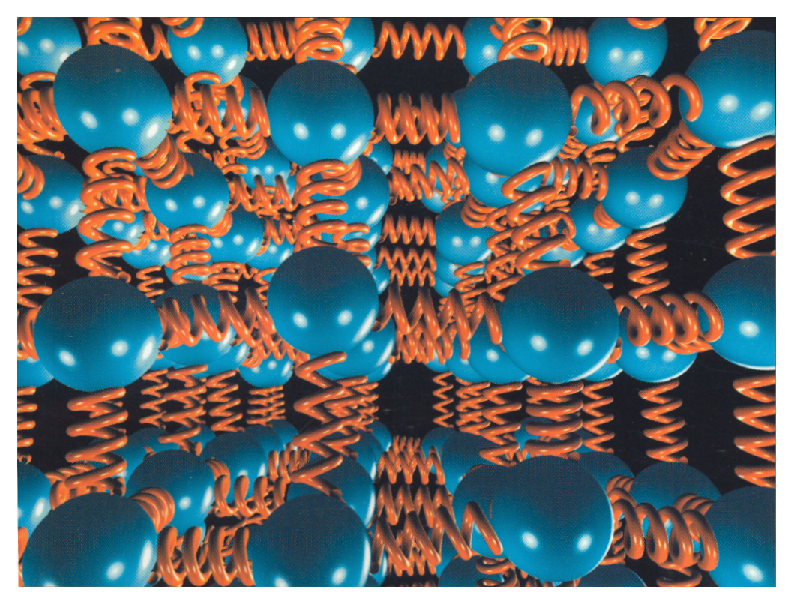
\includegraphics[height=2.0in]{einstein_solid/einstein_solid_picture2.eps}
%
%\hfil Fig. 1 Einstein solid.\hfil 
%
%\setcounter{figure}{1}
%
%\end{wrapfigure}
\begin{equation}
E = \frac{1}{2} m (v_x^2 + v_y^2 + v_z^2) + \frac{1}{2} k (x^2 + y^2 + z^2)
\end{equation}
where $k$ is the spring constant of the bond, the coordinates $x$, $y$, and $z$ are relative to the
equilibrium position of the atom and $v_x$, $v_y$, and $v_z$ are the components of the velocity.
Einstein used an idea pioneered by Max Planck in 1901 and
guessed the energy in the solid came in discrete pieces or quanta that were all
the same size.
Adding or removing these quanta heated or cooled the solid.
Many years later the quantum mechanical energy $E$ for a mass on a spring was found 
to be
\begin{equation}
E = (n_x + n_y + n_z + \frac{3}{2})\hbar \omega
\end{equation}
where $\hbar$ is Planck's constant, $\omega$ is related to the spring constant $k$ of the bond
mentioned
above, and $n_x$, $n_y$, and $n_z$ represent the number of quanta associated with each
degree of freedom of the spring.
The degrees of freedom here correspond to the three possible directions each atom can vibrate.
The size of each energy quantum is $\epsilon = \hbar \omega$.
The total number of energy quanta in the solid is labeled $q_A$ so the internal energy is
$E_{int} = q_A\epsilon$.
We then assume that all microstates of the solid have an equal probability of being populated.
A microstate is a specific arrangement of the quanta on the atoms in the solid.

\textbf{Activity 1: The Statistics of Matter}

Before you embark on building the model of the Einstein solid consider some ideas from
your previous study of gases. 
You will make some predictions here about the statistical nature of matter that you can
refer back to later on in this unit.

(a) Consider a gas in a container. Would it violate Newton's Laws or any other physical law
if all the particles in the gas collided in such a way that all of the gas particles
ended up in the bottom half of the container leaving the top half empty?
\vspace{15mm}

(b) Is such a scenario likely? Explain.
\vspace{15mm}

(c) If you started out with all the gas in the bottom half of the container how likely is
it to stay there?
\vspace{15mm}

The questions you answered above are addressing the notion of irreversibility.
Many processes in nature appear to proceed in one `direction' only.
When you add milk to coffee it disperses throughout the coffee.
After it is dispersed, the milk never re-concentrates into a blob of milk in the
middle of the coffee.
These processes go from a more orderly configuration (a concentrated drop of milk)
to a disordered state (milk spread throughout the liquid).
The reverse never happens.
We will return to this notion again in this laboratory.

\textbf{Activity 2: Calculating the Multiplicity of Some `Solids'}

(a) You will first calculate the configurations of 
the quanta (the microstates) for a VERY simple solid consisting of a single
atom!
The number of atoms for solid $A$ is $N_A=1$ so there are three degrees of
freedom $N_a=3$ because there is one degree of freedom for each
spatial direction.
The atom's vibration can be decomposed into three components, one for each direction.
Let the `solid' contain two quanta of energy so $q_A=2$.
Make a table with the headings $n_1$, $n_2$, and $n_3$ 
and in each row enter one
arrangement of the two quanta.
Each row in the table is a microstate.
Make a table with all of the possible microstates.
The multiplicity $\Omega_A$ of the system is the number of all possible
microstates. What is your multiplicity?
Record it here.
\vspace{45mm}

(b) You can calculate the multiplicity $\Omega_A$ using the expression
\begin{equation}
\Omega(N_A,q_A) = \frac{(q_A + 3N_A -1)!}{q_A! (3N_A-1)!}
\end{equation}
Make the calculation for $N_A = 1$ and $q_A = 2$.
Does this agree with your result in part 2.a?
\vspace{15mm}

(c) Now do the same thing for a different `solid'.
This time for solid $B$, let $N_B = 2$ (two whole atoms!) and $q_B = 1$.
How many degrees of freedom does solid $B$ have?
Make a table analogous to the one in part 2.a on the same sheet as before.
What is the multiplicity of solid $B$?
Record it here.
Use the expression in Activity 2.b to check your calculation.
\vspace{45mm}

\textbf{Activity 3: Putting the `Solids' Together}

When two solids are brought together heat/energy can flow between the two objects.
For the model of the Einstein solid you are building this corresponds to 
energy quanta ($\hbar \omega$) moving from atom to atom and occupying different
microstates of the combined system.

(a) Now bring the your solids $A$ and $B$ `together' into a single system.
What is $N_{AB}$ the total number of atoms?
What is the number of degrees of freedom of the combined system?
\vspace{10mm}

(b) What is the total number of energy quanta $q_{AB}$ for the combined system?
\vspace{10mm}

(c) The system is in its initial macrostate.
A macrostate is a configuration of the system defined here by the total number
of atoms and quanta in each solid.
In this case the macrostate is defined by $N_A=1$, $q_A=2$, $N_B=2$, and $q_B= 1$.
 What is the total multiplicity $\Omega_{AB}$ for the combined system
with $q_A=2$ and $q_B=1$ in its initial macrostate?
\vspace{15mm}

(d) Now take the energy quantum in solid $B$ and put it in solid $A$,
{\it i.e.}, let heat flow from solid $B$ into solid $A$.
This is now a macrostate where $q_A=3$ and $q_B=0$.
What is the new multiplicity $\Omega_A$ for solid $A$ and the  multiplicity $\Omega_B$ for solid $B$?
\vspace{20mm}

(e) What is the multiplicity $\Omega_{AB}$ for the combined system (solids $A$ and $B$)?
\vspace{15mm}

(f) Remember that a macrostate is defined by the combination of $N_A$, $N_B$, $q_A$, and $q_B$.
Which macrostate had the greatest multiplicity, $(q_A=2, ~ q_B=1)$ or $(q_A=3, ~ q_B=0)$
(remember that $N_A$ and $N_B$ are the same in each configuration so we don't 
list those parameters here)?
\vspace{15mm}

(g) If the energy quanta can move from atom to atom
which macrostate $(q_A=2, ~ q_B=1)$ or $(q_A=3, ~ q_B=0)$ is most probable? Why?
\vspace{15mm}

(h) If you started out in the $(q_A=3, ~ q_B=0)$ macrostate is it more likely that you will remain
in that macrostate of evolve to the $(q_A=2, ~ q_B=1)$ macrostate? Why?
\vspace{15mm}

What you have discovered is a version of the irreversibility mentioned earlier,
One macrostate ($q_A=2$, $q_B=1$) is preferred over the other because it has more microstates
than the other.
This result depends critically on your assumption that all states are equally populated.

\newpage

\textbf{Activity 4: Using {\it StatMech} For More Complex Cases}

You should have found in the previous activity that the $(q_A=2, ~ q_B=1)$ 
macrostate was more likely
to occur and the process proposed in part 3.d is relatively unlikely.
In other words, it is more likely for energy to be spread evenly throughout the system.
This is good news because it means the statistical picture we are painting is consistent
with reality.
Remember what happens to the blob of milk in the coffee.

(a) You should realize that making the sorts of calculations you did in Activity 3 above would
become rather painful for say $N_A = 300$ atoms.
In order to push the model further you will use a software packaged called 
{\it StatMech} to perform the same calculations.
To run the program go to the {\tt Physics Applications} menu and click on
{\tt StatMech}.
You should see a window like the one below.
\begin{figure}[!ht]
\begin{center}
\includegraphics[height=4.0in]{einstein_solid/statmech1.eps}
\caption{The {\tt StatMech} window showing the table of multiplicities for each microstate.
Each row corresponds to a different value of $q_A$.}
\index{color page}
\end{center}
\end{figure}
The top of the window has several entry boxes where you can set the number of
atoms ($N_A$ and $N_B$) and the total number of energy quanta in the system $U$.
The parameter $U$ is the total internal energy $_{int}$ in the system in 
units of $\epsilon = \hbar \omega$.
It is equivalent to the sum $q_{AB} = q_A + q_B$.
You can also set the number of rows of microstates to print out
or choose to view a graph instead of the table.
To test the operation of {\it StatMech} redo the calculations of the microstates that
you did in Activity 3. Make sure your results in Activity 3 agree with the output of 
{\it StatMech}.
You will also see there are other macrostates that were ignored in Activity 3 for
simplicity.

(b) Now run {\it StatMech} for the case where $N_A = 10$, $N_B=20$, $U = 500$.
What is the value of $q_A$ for the most probable macrostate? 
%qA = 165.
Record it here.
Click on the button at the top of the {\it StatMech} window and choose graph.
You will see a graph of the table  and it should look something like
Figure 2.
\begin{figure}[!ht]
\begin{center}
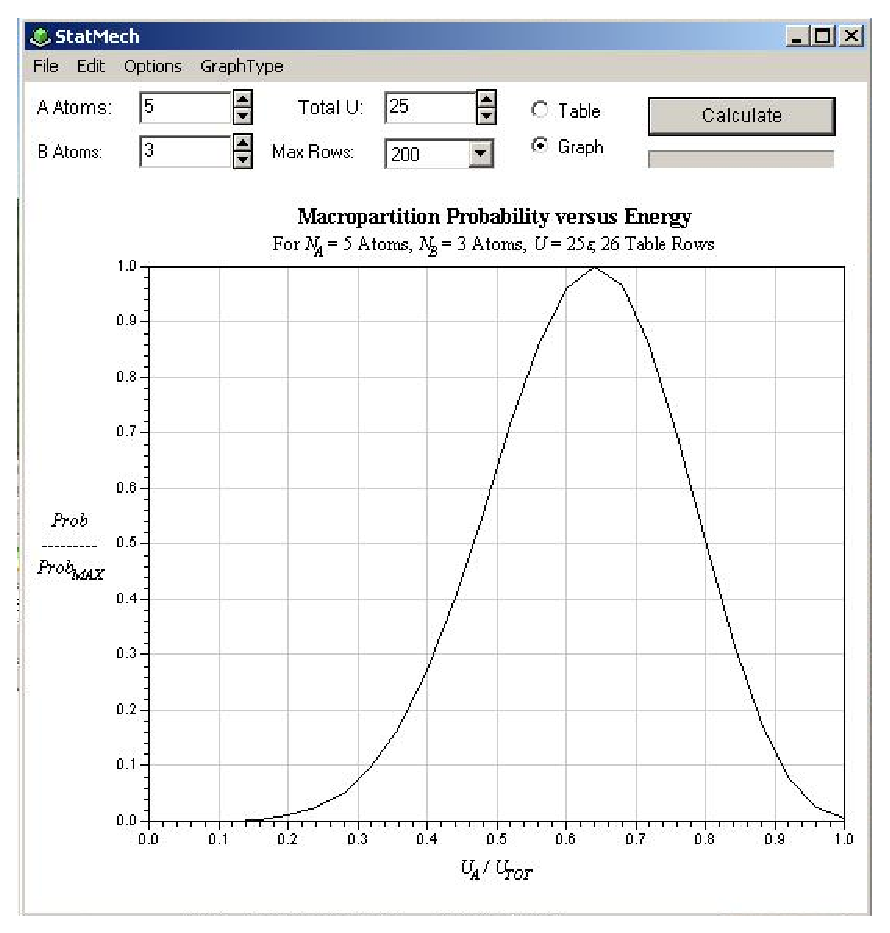
\includegraphics[height=4.0in]{einstein_solid/statmech2.eps}
\caption{The {\tt StatMech} window showing a graph of the multiplicities as a function
of $E_A/E_{int}$ where $E_A = q_A \hbar \omega$ and 
$E_{int} = q_{AB} \hbar \omega = (q_A+q_B)\hbar \omega$.}
\index{color page}
\end{center}
\end{figure}
The vertical axis is the probability of a particular macrostate divided by the maximum
probability of any macrostate.
The horizontal axis is  $U_A/U_{TOT}$ where 
$U_A$ is the energy of solid $A$ in units of $\epsilon$ (equivalent to $q_A$) and $U_{TOT}$ is the total
internal energy of the solid in units of $\epsilon$ (equivalent 
to the total number of quanta $q_{AB}$).
What is the value of $U_A/U_{TOT}$ for the most probable state?
How is this value related to the value of $q_A$ for the most probable macrostate? 
Also, explain in words what this plot is showing you.
\vspace{25mm}

(c) How wide is the distribution of microstates?
Measure this number by estimating the full-width-half-maximum (FWHM) from your graph.
Do this by finding the largest value on the vertical axis, divide that value by two, and find
the two points on either side of the peak where the distribution is equal to that
half-maximum.
Take the difference between these two points along the horizontal and this is the FWHM.
Record your result here.
%$U_A/U_{TOT} = 0.32
% sigma = 0.39-0.26 = 0.13
\answerspace{20mm}

(d) Now repeat steps 4.b-c with $U=100,000$ and $N_A$ and $N_B$ at their last values.
What is the most probable value of $U_A/U_{TOT}$ and the FWHM?
How have things changed?
%$E_A/U_{TOT} = 0.32
% sigma = 0.39-0.26 = 0.13
\answerspace{25mm}

\pagebreak[3]
(e) Keeping $U=100,000$ now repeat steps 4.b-c, but this time double the values of $N_A$ and $N_B$.
Record the most probable macrostate and the FWHM.
Repeat this doubling of the number of atoms in each solid while keeping $U$ fixed at least 3-4 times.
Record the most probable macrostate and the FWHM each time along with $N_A$ and $N_B$.
% 10:20 peak=0.32 sigma=0.13
% 20:40 peak=0.32 sigma=0.38-0.29=0.09
% 40:80 peak=0.32 sigma=0.36-0.30=0.06
% 80:160 peak=0.32 sigma=0.35-0.31=0.04
% 160:320 peak=0.32 sigma=0.34-0.32=0.02
\vspace{45mm}

(f) How does the value of $q_A$ for the most probable macrostate change as the number
of atoms increases?
\vspace{15mm}

(g) How does the FWHM change as the number of atoms increases?
\vspace{15mm}

\textbf{Activity 5: Irreversibility}

You will now use the results from the previous Activity to delve into some of the
implications of the statistical mechanics of the Einstein solid.

(a) As the number of atoms increases, what happens to the probability for finding the
system in a macrostate different from the most probable one?
Use the results of your calculations to explain your answer.
\vspace{15mm}

(b) When the system is in a macrostate far from the most probable one, what is the most
likely thing to happen as energy or heat flows around the system?
\vspace{15mm}

(c) For the last calculation in Activity 4 
what is the probability of the state with the minimum value of $q_A$?
%10^-813
In other words what is the probability that all of the quanta would end up all in solid $B$?
What is the probability of the most probable macrostate?
%qA=334, frac = 0.03186
\vspace{15mm}

(d) Go back to the questions in Activity 1 and look at your answers. 
Do they still appear to be correct?
A situation where all of the gas particles end up in one part of the container is a macrostate
of the system analogous
to the situation in Activity 5.c where all of the quanta end up in one  of the solids and 
not the other.
Answer those questions in Activity 1 again in terms of microstates, macrostates, and probability.

The behavior you are seeing here is for an Einstein solid, but is actually typical for
most macroscopic systems. These systems have a large number of atoms or molecules
with a variety of different energy states available.
They evolve to the most probable macrostate and there is essentially no chance to occupy a state
far from the most probable one. 
When two materials are first put in thermal contact they may be far from the most probable 
macrostate, but they equilibrate at that most probable one (where the temperatures are equal)
and never go back.
This is irreversibility.

%\vspace{15mm}


\bigskip

\textbf{Activity 6: Homework Problems} (E - exercise, P - problem)

\begin{enumerate}

\item(E) Consider the following `gas'.
It consists of four atoms in a cubical box. At any instant, there is a 50\% chance
of each atom being in the left half of the box ($L$) or the right half ($R$).
Make a table showing all the microstates of this system. (Hint: There are 16.)
How many macrostates are there?
How many microstates are in each macrostate?

\item (E) Show that for $N$ gas atoms in a box, the number of possible microstates is
$2^N$ when microstates are defined by whether a given molecule is in the left half
of the box or the right half of the box.
The volumes of each half are equal.


\item (E) Imagine that we have an ideal gas consisting of 15 molecules.  
We can flip the signs of each of the three velocity components of a given molecule w
without changing its overall energy (and thus without changing the gas's macrostate).  
How many possible patterns of sign choices are there?

\item (E) Calculate the multiplicity of an Einstein solid with $N = 1$ and $E_{int} = 6\epsilon$ 
by directly listing and counting the microstates.  
Check your work by using equation 3.

\item (E) Calculate the multiplicity of an Einstein solid with $N = 1$ and 
$E_{int} = 5\epsilon$  by directly listing and counting the microstates.  
Check your work by using equation 3.

\item (E) Use equation 3 to calculate the multiplicity of an 
Einstein solid with $N = 4$ and $E_{int} = 10\epsilon$.

\item (E) Use equation 3 to calculate the multiplicity of an 
Einstein solid with $N = 3$ and $E_{int} = 15\epsilon$.

\item (E) How many times more likely is that the combined system of 
solids described in the table below will be found in macropartition 3:3 than 
in macropartition 0:6, if the fundamental assumption is true?

\item (E) How many times more likely is it that the combined system of 
solids describe in the table below will not be found in macropartition 3:3 
than it is to be found in macropartition 0:6, if the fundamental assumption is true?

\begin{table}[hbt!]
\begin{center}
\begin{tabular}{|lccccc|} \hline
\hi Macropartition  & $E_A$ & $E_B$ & $\Omega_A$ & $\Omega_B$ & $\Omega_{AB}$ \\[5pt] \hline
\hi 0:6             & 0     & 6     & 1          & 28         & 28            \\[5pt]
\hi 1:5             & 1     & 5     & 3          & 21         & 63            \\[5pt]
\hi 2:4             & 2     & 4     & 6          & 15         & 90            \\[5pt]
\hi 3:3             & 3     & 3     & 10         & 10         & 100            \\[5pt]
\hi 4:2             & 4     & 2     & 15         & 6          & 90           \\[5pt]
\hi 5:1             & 5     & 1     & 21         & 3          & 63            \\[5pt]
\hi 6:0             & 6     & 9     & 28         & 1          & 28           \\[5pt] \hline
\hi                 &       &       &            & Total=     & 462         \\[5pt] \hline
\end{tabular}
\end{center}
\caption{Possible macropartitions for $N_A=1$, $N_B=1$, $E_{int}=6\epsilon$.}
\end{table}

\item (E) Consider the system consisting of a pair of Einstein solids in thermal contact.  
A certain macropartition has a multiplicity of $3.7 \times 10^{1024}$, while the total number of 
microstates available to the system in all macropartitions is $5.9 \times 10^{1042}$.  If we look 
at the system at a given instant of time, what is the probability that we will find it 
to be in our certain macropartition?

\item (E) Consider the system consisting of a pair of Einstein solids in thermal contact.  
A certain macropartition has a multiplicity of $1.2\times 10^{346}$, while the total number of 
microstates available to the system in all macropartitions is $5.9 \times 10^{362}$.  If we look 
at the system at a given instant of time, what is the probability that we will find it 
to be in our certain macropartition?

\item (E) Consider the system consisting of a pair of Einstein solids in thermal contact.  
Imagine that it is initially in a macropartition that has a multiplicity of $8.8 \times 10^{123}$.  
The adjacent macrostate closer to the equilibrium macrostate has a multiplicity
of $4.2 \times 10^{1234}$.  If we look at the system a 
short later, how many times more likely is it to have moved to the second macropartition 
than to have stayed with the first?

\item (E) Consider the system consisting of a pair of Einstein solids in thermal contact.  
Imagine that it is initially in a macropartition that has a multiplicity of $7.6 \times 10^{3235}$.  
The adjacent macropartition closer to the equilibrium macropartition has a multiplicity 
of $4.1 \times 10^{3278}$.  If we look at the system a short time later, how many times more likely 
is it to have moved to the second macropartition than to have stayed with the first?

\item(P) Suppose you put 100 pennies in a cup, shake it up, and toss them all into the
air.
(a) After landing, how many different head-tail arrangements (microstates) are possible for
the hundred pennies?
(b) What is the probability of finding exactly 50 heads? 
(c) 49 heads?
(d) 1 head?

\item(P) You ask your roommate to clean up a mess he or she made in your room.  Your roommate 
refuses, because cleaning up the mess would violate the second law of thermodynamics, and 
campus security's record of your roommate's legal violation is already excessive.  
Gently but firmly explain why complying will not put your roommate at risk of such an infraction.

\item(P) The classic statement of Murphy's law reads, `If something can go wrong, it will.'   
Explain how this is really a consequence of the second law of thermodynamics.  (Hint:  
What is the entropy of `wrong' in a given context compared to the entropy of `right'?)

\item(P) Run the {\it StatMech} program to answer the questions below.

\begin{enumerate}

\item For two Einstein solids in contact with 
$N_A = N_B = 100$ and 
$E_{int} = 200\epsilon$ answer the following questions.  (1) How many times more likely is the system 
to be found in the center macropartition than in the extreme macropartition where $E_A = 0$ 
and $E_B = 200\epsilon$ 
(2) What is the range of values that $E_A$ is likely to have more than 99.98\% 
of the time?  (3) if $E_A$ were initially to have the extreme value 0, how many times more 
likely is it to move to the next macropartition nearer the center than to remain in the 
extreme one?
\item  Answer the same question as in (a) for a run where you scale everything up by a 
factor of 10, so that $N_A = N_B = 1000$ and $E_{int} = 2000\epsilon$.
\item  Answer the same question as in (a) for a run where $N_A = N_B = 1000$ and 
$E_{int} = 200\epsilon$.  
Comment on the effect that increasing just the size of the system by a factor of 10 
has on these answers.
\item Answer the same question as in (a) for a run where $N_A = N_B = 100$ and $E_{int} = 2000\epsilon$.  
Comment on the effect that increasing just the energy available to the system by a factor 
of 10 has on these answers.

\end{enumerate}

\item(P) Consider two Einstein solids in thermal contact.  The solids have different 
values of N but are identical in all other respects.  It is plausible, since every atom 
in the combined system is identical, that in equilibrium the energy will be distributed 
among the solids in such a way that the average energy per atom is the same.  Use {\it StatMech} 
to test this hypothesis in the situation where $E_{int} = 1000\epsilon$ and $N_A$ and $N_B$ have various 
different values such that $N_A + N_B = 1000$.  (Set {\tt Max Rows} to 1000 so that you can see 
every macropartition).
\begin{enumerate}
\item Is it true in most cases that in the most probable macropartition the solids have 
energies such that the average energy per atom in each is the same?  Is it strictly 
true in every case?  Answer these questions by discussing the values $N_A$ and $N_B$ you tested, 
and whether the actual most probable macropartition is the same as that predicted by the hypothesis.
\item In any case where the hypothesis does not work, does increasing both $N_A$ and $N_B$ by a 
factor of 10 or 100 (but leaving $U$ alone) yield a result more or less consistent with 
the hypothesis?
\item Speculate as to the value of this hypothesis in the large-$N$ limit.
\end{enumerate}
\item(P) For the following questions, you will find that using {\it StatMech} is 
by far the fastest way to calculate the multiplicity.
\begin{enumerate}
\item  What is the entropy of an Einstein solid with 5 atoms and an energy of 
$15\epsilon$?  Express your answer as a multiple of $k_b$.
\item  What is the entropy of an Einstein solid with 50 atoms and an energy of $100\epsilon$?  
Express your answer as a multiple of $k_b$.
\end{enumerate}

\item(P) A certain macropartition of two Einstein solids has an entropy of $305.2k_b$.  
The next macropartition closer to the most probable one has an entropy of $335.5k_b$.  
If the system is initially in the first macropartition and we check it again later, 
how many times more likely is it to have moved to the other than to have stayed in the first?

\item(P) My calculator cannot display $e^x$ for $x> 230$.  One can calculate $e^x$ for larger 
values of $x$ as follows.  Define $y$ such that $x = y \ln 10$.  This means that 
$e^x = e^{y\ln 10} = (e^{\ln10})^y = 10^y = 10^{x\ln 10}$.  
Note that we can calculate 10 raised to a 
non-integer power (for example, 103.46) as follows:  
$10^{3.46} = 10^{3+0.46} = 10^3(10^{0.46}) = 2.9 \times 10^3$.  
Use these techniques to solve the following problem.  The entropy of the most probably 
macropartition for a certain system of Einstein solids is $6025.3k_b$, while the entropy 
of an extreme macropartition is only $5755.4k_b$.  What is the probability of finding the 
system at a given time in the extreme macropartition compared to that of finding it in 
the most probable macropartition?

\item(P) In principle, the entropy of a isolated system decreases a little bit whenever 
random processes cause its macropartition to fluctuate away from the most probable 
macropartition.  We can certainly see this with small systems. 
But is this really a possibility for a typical macroscopic system?  Imagine that 
we can measure the entropy of a system of two solids to within 2 parts in 1 billion.  
This means that we could just barely distinguish a system that has an entropy of 
4.99999999 J/K (eight 9s!) from one that has 5.00000000 J/K.  (This is a reasonable 
entropy for a macroscopic system).
\begin{enumerate}
\item Imagine that the entropy of the equilibrium macropartition is 5.00000000 J/K.  
Show that the approximate probability that at any given time later we will find the 
system in a macropartition with entropy 4.99999999 J/K ({\it i.e.}, with an entropy that 
is only barely measurably smaller) is about 10315,000,000,000,000 times smaller that 
the probability we will still find it to have entropy 5.00000000 J/K. (Hint:  See problem 17.)
\item Defend the statement that the entropy of an isolated system in thermal equilibrium 
never decreases.
\end{enumerate}

\end{enumerate}




\section{Entropy and Temperature}

\makelabheader %(Space for student name, etc., defined in master.tex)

\textbf{Objective}

To explore the connection between the fundamental definition of entropy and
temperature.

\textbf{Overview}

Consider the microscopic  definition of the entropy of a system
\begin{equation}
S = k_B \ln \Omega
\end{equation}
where $k_B$ is Boltzmann's constant and $\Omega$ is the multiplicity or number of 
microstates.
A microstate is defined by a particular arrangement of energy quanta among the
atoms.
A macrostate is defined by the total number of energy quanta $q$ and the number of atoms $N$.
We are building a model of an elemental solid ({\it e.g.}, like aluminum)
where
the total internal energy in the solid $E_{int}$ is described by
\begin{equation}
E_{int} = q \hbar \omega 
\end{equation}
where $\hbar$ is Planck's constant divided by $2\pi$ and $\omega$ is a constant that
characterizes the strength of the bonds between the atoms.
The parameter 
$q$ is the total number of quanta in the system and is a constant.
These quanta are statistically distributed over the $N$ atoms of the solid so
all possible states of the system are equally likely and the multiplicity $\Omega$
is
\begin{equation}
\Omega = \frac{(q+3N-1)!}{q!(3N-1)!} \qquad .
\end{equation}
This model of an elemental solid is called an Einstein solid.

We want to find a connection between the entropy defined in Equation 1 and the
temperature.
Recall how temperature is usually defined
relative to some properties of matter like the freezing and 
boiling points of water.
You are developing the microscopic picture of entropy, but it won't be successful until
you can connect it to the observed behavior of bulk matter and our familiar notions of 
temperature.

\textbf{Activity 1: The Entropy of Einstein Solids in Thermal Equilibrium}

(a) To start connecting the entropy to the temperature you have to study the 
behavior of the entropy as the energy changes.
To do this we will study two Einstein solids ($A$ and $B$) in thermal equilibrium with 
each other.
Their total internal energy will be
\begin{equation}
E_{int} = q_{AB}\hbar \omega = (q_A + q_B) \hbar \omega
\end{equation}
where $q_A$ and $q_B$ are the numbers of energy quanta in each solid and $q_{AB}$ is 
their sum.

Use the program {\it StatMech} (see the {\tt Physics Applications} menu)
for the configuration where you choose $N_A > 100$, $N_B > 80$ and $U>400$.
The label $U$ in the {\it StatMech} window refers to the total number of energy quanta 
in the system
in units of $\hbar \omega$ and is equivalent to $q_{AB}$ here.
An example of the output of {\it StatMech} is shown in Figure 1.
\begin{figure}[ht!]
\begin{center}
\includegraphics[height=4.0in]{entropy_temperature/statmech1.eps}
\caption{The {\tt StatMech} window showing the table of multiplicities for each microstate.
\index{color page}
Each row corresponds to a different value of $q_A$.}
\end{center}
\end{figure}
The first two columns in the lower panel of Figure 1 represent $U(A)$ and $U(B)$, 
the energies in each 
individual solid (again in units of $\hbar \omega$) and are equivalent to $q_A$ and $q_B$.
After you perform the calculation with {\it StatMech} scan quickly down the column
labeled `Omega(AB)'.
If any of the exponents you see exceed the value 307, then run the calculation again with 
smaller inputs until no exponent exceeds 307.
This limitation is a restriction on MicroSoft {\it Excel} that you will use later to make
plots.
Record your values of $N_A$, $N_B$, and $U$.
\vspace{15mm}

(b) Now generate plots of $S_{AB}=S_A + S_B$, $S_A$, and $S_B$ from the {\it StatMech} table.
You can do this with {\it Excel}, but there are some intermediate steps necessary.
Start Microsoft {\it Word} first.
Next, go to the {\it StatMech} window, highlight the table, copy it
 (see the {\tt Edit} menu on the {\it StatMech} window), and paste it into the {\it Word}
document. 
In {\it Word} edit out all the commas (`,') and asterisks (`*') in the file 
(use the {\tt Replace}
option under the {\tt Edit} menu).
Save the Word file, but save it as a plain text (`\*.txt') file.
You can now open the file in {\it Excel}.
When you open the file, {\it Excel} pops up a {\tt Text Import Wizard} 
that will guide you through
the format of the input file.
The defaults usually seem to work.
Use {\it Excel} to calculate and plot on one graph $S_{AB}$, $S_A$, and $S_B$
as a function of $q_A$.
Print out your plot and attach it to this unit.

(c) What is $q_A$ for the most probable macrostate? What mathematical condition can you impose
on the total entropy $S_{AB}$ to determine the most probable macrostate?
How do you think the temperatures of solids $A$ and $B$ are related at the most probable 
microstate?
\vspace{15mm}

(d) How are the slopes of $S_A$ and $S_B$ related to one another at the most probable
macrostate?
\vspace{30mm}

\newpage

(e) How is $E_A$, the energy in solid $A$ related to $q_A$?
How is $E_B$, the energy in solid $B$ related to $q_A$?
Remember that $q_{AB}$ is a constant and $q_{AB} = q_A + q_B$.
Calculate the differentials $dE_A$ and $dE_B$ and rewrite the answer in part 1.d
in terms of $dS_A/dE_A$ and $dS_B/dE_B$.
\vspace{45mm}

\textbf{Activity 2: Relating Entropy and Temperature}

(a) Using the spreadsheet you generated in Activity 1, calculate $dS_A/dq_A$ as a function
of $q_A$ and plot it. You can do this to an adequate approximation
by doing taking the difference between $S_A$ at adjacent values/rows
of $q_A$.
To do this suppose your spreadsheet has the values of $S_A$ in column $H$.
The {\it Excel} syntax for estimating the derivative for the first value of
$q_A$ (the first row) is 
`{\tt =(H2-H1)/1.0}' where {\tt H2} is the value in the second row and {\tt H1} is the
value in the first row.
The numerator of one is redundant, but it shows you are approximating the derivative
using the data from points that differ by 1.0 in $q_A$, the number of quanta in solid $A$.
The syntax for $dS_A/dq_A$ for the second value of $q_A$ is `{\tt =(H3-H2)/1.0}' and so on.
Do the same for $dS_B/dq_A$ and $dS_{AB}/dq_A$.
Does the slope of $S_{AB}$ pass through zero at the correct spot (recall part 1.c)?
How are $dS_A/dq_A$ and $dS_B/dq_A$ related at the most probable macrostate.
Does you plot agree with that result?
\vspace{15mm}

(b) If the energy $E_A$ and $q_A$ of solid $A$ increases what should the temperature 
of solid $A$ do?
If the energy $E_A$ of solid $A$ increases what happens to $dS_A/dq_A$ in your plot?
Do the temperature and $dS_A/dq_A$ change in the same  way or in a different way 
as $E_A$ increases?
\vspace{15mm}

(c) We want to come up with a relationship between temperature and the entropy.
From the results above (parts 1.a-e) you should have found
\begin{equation}
\frac{dS_A}{dE_A} = \frac{dS_B}{dE_B}
\end{equation}
and
\begin{equation}
T_A = T_B
\end{equation}
for the most probable macrostate.
This means there is some function of the temperature $T$ such that
\begin{equation}
f(T) = \frac{dS}{dE}
\end{equation}
for each solid that will be equal at equilibrium.
We want $f(T)$ to behave like the temperatures we are accustomed to using.
In other words, as the energy in the solid increases $T$ should increase.
Recall part 2.b and the behavior of $dS/dE$ as $T$ increases.
Try to guess a mathematical form of $f(T)$ that acts like `normal' temperatures
and one that doesn't. Explain your reasoning.
\vspace{30mm}

(d) How would you choose which of the forms you guessed in part 2.c is the correct one?
\vspace{15mm}

\textbf{Activity 3: Determining $f(T)$ and the Heat Capacity}

In the previous Activity you should have found that the mathematical form of $f(T)$
has to be something like $1/T^n$ where $n$ is some positive number.
This is necessary because your graphs should show that as the energy $E_A$ (and the number
of quanta $q_A$) of the solid 
increases $f(T)=dS/dE$ goes down. To make sure the temperature $T$ behaves reasonable
(and goes up with $E_A$ and $q_A$) $f(T)$ must be some inverse of function of $T$.
To decide exactly which function is right requires comparing Equation 7 or some
result from it to some data.

Recall the table of heat capacities we generated in the laboratory entitled
{\it Calorimetry}.
Use those results to fill in Table 1 making sure that you are using molar 
heat capacities.
\begin{table}
\begin{center}
\begin{tabular}{|p{0.8in}|l|p{0.8in}|l|} \hline
\hi Solid    & $dE/dT$ per mole & Solid      & $dE/dT$ per mole   \\[2pt] \hline
\hi          &                  &            &       \\[2pt] \hline
\hi          &                  &            &      \\[2pt] \hline
\hi          &                  &            &      \\[2pt] \hline
\end{tabular}
\caption{Molar specific heats ($(1/n)dE/dT$) for several elemental solids.}
\end{center}
\end{table}
%Consider Table 1 of heat capacities ($dE/dT$) for several elemental solids
%for high temperatures.
%\begin{table}
%\begin{center}
%\begin{tabular}{|p{0.8in}|l|p{0.8in}|l|} \hline
%\hi Solid    & $dE/dT$ per mole & Solid      & $dE/dT$ per mole   \\[2pt] \hline
%\hi Lead     & $26.4~J/K-mole$    & Gold     & $25.4~J/K-mole$      \\[2pt]
%\hi Silver   & $25.4~J/K-mole$    & Copper   & $24.5~J/K-mole$      \\[2pt]
%\hi Iron     & $25.0~J/K-mole$    & Aluminum & $26.4~J/K-mole$      \\[2pt] \hline
%\end{tabular}
%\caption{Heat capacities ($dE/dT$) for several elemental solids.}
%\end{center}
%\end{table}
 The heat capacities are constant with respect to temperature and are similar in value to
one another.
These are the data that will help us determine $f(T)$.
To calculate $dE/dT$ we must find a relationship between $E$ and $T$ for the Einstein solid.

(a) Start with Equations 1 and 7 and the chain rule and show the following.
\begin{equation}
\frac{dS}{dE} = k_B \frac{1}{\Omega} \frac{d\Omega}{dE}
\end{equation}
\vspace{15mm}

(b) Use Equation 2 to show 
\begin{equation}
dE = \hbar \omega dq \qquad {\rm and} \qquad  
    \frac{d\Omega}{dE}=\frac{1}{\hbar\omega} \frac{d\Omega}{dq}
\qquad .
\end{equation}
\vspace{15mm}

\newpage

(c) Starting with Equations 1 and 3 one can show
\begin{equation}
\frac{d\Omega}{dq} = \frac{3N\hbar \omega}{E} \Omega
\qquad .
\end{equation}
Combine this equation (number 10) and the  results from 3.a-b to 
get a relationship for $dS/dE$ for the Einstein solid in terms
of $N$ and $E$.
Set that expression equal to $f(T)$,
and solve for $E$ the internal energy.
It is the derivative of this last equation ($(1/n)dE/dT$) that will give you the molar specific heat.
What function of $f(T)$ will give a result that is independent of temperature when you
take the derivative with respect to $T$ of your expression for the internal energy $E$?
\vspace{45mm}

(d)  What is the final form of Equation 7 and $f(T)$?
\vspace{15mm}

(e) Determine the mean and standard deviation of the heat capacity of the elemental solids in
Table 1.
Calculate the molar specific heat ($(1/n)dE/dT$) for the Einstein solid using your results from
parts 3.c-d.
Is the molar specific heat for the model of the Einstein solid consistent with the measured ones?
\vspace{45mm}


\textbf{Activity 4: The Second Law of Thermodynamics}

(a) Go back to your plots of the entropy as a function of $q_A$ from part 1.b. 
Consider two Einstein solids that are brought together at a value of $q_A$ that is higher
than the equilibrium one at the most probable macrostate.
Choose a value of $q_A$ that is halfway between the most probable value and the maximum.
Once the two Einstein solids are in contact, how will the system evolve?
What happens to $S_A$ and $S_B$? Do they go up, down, or stay the same?
What happens to the total entropy $S_{AB}$?
In fact, based on your plot from part 2.b, is there any circumstance where
$S_{AB}$ will not increase?
\vspace{30mm}

(c) To  vividly see what happens when Einstein solids come in thermal contact,
run the program {\it equilib.exe} available in the {\tt Physics Applications} menu.
This program starts with two Einstein solids with all the energy quanta in solid $B$.
It simulates the evolution of the two solids as they march toward
thermal equilibrium.
Click {\tt Evolve} to see the simulation run.

What you should have discovered in the previous part is that the entropy of the combined systems
always increases regardless of what configuration the Einstein solids are in when they
come in contact.
The system always evolves to the most probable, most disordered
 macrostate where the temperatures will
be equal and the entropy is a maximum.
The energy quanta are most spread out.
This result is stated in several different ways, but the most succinct is simply
$\Delta S > 0$ for an isolated system.
The entropy of an isolated system always increases.
This is called the Second Law of Thermodynamics.

\bigskip

\textbf{Activity 4: Homework Problems}

\begin{enumerate}
 
\item (E) An object's entropy is measured to increase by $0.1~ J/K$ 
when we add $35~ J$ of energy.  What is its approximate temperature?  
(Assume that the object's temperature does not change much when we add the $35~J$.)

\item (E) A certain Einstein solid's entropy changes from 
$305.2k_b$ to $338.1k_b$ when we add 1 unit $\epsilon$ of energy.  
What is the value (and units) of $k_bT/\epsilon$ for this solid?  
If $\epsilon = 1.0~eV$, what is its temperature $T$?

\item (E) Does it make sense to talk about the 
temperature of a vacuum?  If so, how could you measure or calculate it?  
If not, why not?  

\item (E) An Einstein solid in a certain macrostate has a multiplicity of $3.8 \times 10^{280}$.  
What is its entropy (expressed as a multiple of $k_B$)?

\item (E) A pair of Einstein solids in a certain macropartition has multiplicities of 
$4.2 \times 10^{320}$ and $8.6 \times 10^{132}$.  What are the entropies of 
each solid?  What is the total 
entropy of the system in this macropartition?  (Express entropies as multiples of $k_b$.)

\item (E) Is it really true that the entropy of an isolated system consisting of two 
Einstein solids never decreases?  (Consider a pair of very small solids.)  Why is this 
statement more accurate for large systems than for small systems?  Explain in your own words.

\item (P) In lab we argued on fairly fundamental grounds 
that $dS/dU = f(T)$.  In principle, we could define $f(T)$ to be anything 
that we like:  this would amount to defining temperature and its scale. 
Still, some definitions would violate deeply embedded preconceptions 
about the nature of temperature.  
For example, the simplest definition of temperature would be $dS/dU = T_{new}$.  
Show that this definition
\begin{enumerate}
\item Would imply that $T_{new}$ has units of $K^{-1}$ and
\item Would imply that heat would flow spontaneously from objects with 
low $T_{new}$ to objects with high $T_{new}$.  
This would imply that object with low values of $T_{new}$ are hot, while 
objects with high values $T_{new}$ are cold (we might want to call $T_{new}$ 
so defined {\it coolness} instead of {\it temperature}).  
While we could define temperature in this way, it would really fly 
in the face of convention (if not intuition).
\item If we did define coolness $T_{new}$ in this way, what ordinary 
temperature $T$ would an object with absolutely zero coolness (
$T_{new} = 0$) have?  What about something that is infinitely cool ($T_{new} = \infty$)?
\end{enumerate}

\item (P) Imagine that the entropy of a certain substance as a function of 
$N$ and $U$ is given by the formula $S = Nk_b \ln U$. Using the definition of temperature, 
show that the thermal energy of this substance is related to its temperature 
by the expression $U=Nk_b T$.

\item (P) Imagine that the multiplicity of a certain substance is 
given by $\Omega(U,N) = Ne^{\sqrt{NU/\epsilon}}$, where $\epsilon$ is some unit of energy.  
How would the energy of an object made out of this substance depend 
on its temperature?  Would this be a `normal' substance in our usual sense 
of temperature.

\item (P) Consider an Einstein solid having $N = 20$ atoms.  
\begin{enumerate}
\item What is the solids temperature when it has an energy of $10\epsilon$, 
assuming that $\epsilon =h\omega = 0.02 eV$?  Calculate this directly from the 
definition of temperature by finding $S$ at $10\epsilon$ and $11\epsilon$, computing 
$dS/dU \approx [S(11\epsilon) - S(10\epsilon)]/\epsilon$, and then applying 
the definition of temperature.  (You will find that your work will 
go faster if you use {\it StatMech} to tabulate the multiplicities.)
\item How does this compare with the result from the formula $U = 3Nk_bT$ 
(which is only accurate if $N$ is large and $U/3N\epsilon > 1$)?
\item If you have access to {\it StatMech}, repeat for 
$N = 200$ and $U =100\epsilon$.  
(Hint:  If your calculator cannot handle numbers in excess of $10^{100}$, 
use the fact that in $(a \times 10^b) = \ln a + b \ln 10 $).
\end{enumerate}

\item (P)  A newly-created material has a multiplicity
$$
\Omega = \alpha N E
$$
where $N$ is the number of atoms in the solid,
$E$ is the total, internal energy in the solid, and $\alpha$ is a constant of 
proportionality.
\begin{enumerate}
\item How does the temperature of the new material depend on the internal energy?
\item What is the molar heat capacity for this solid?
\item Could this material really exist? Why or why not?
\end{enumerate}

\item (P)  A newly-created material has a multiplicity
$$
\Omega = \beta M E^2
$$
where $N$ is the number of atoms in the solid,
$E$ is the total, internal energy in the solid, and $\alpha$ is a constant of 
proportionality.
\begin{enumerate}
\item How does the temperature of the new material depend on the internal energy?
\item What is the molar heat capacity for this solid?
\item Could this material really exist? Why or why not?
\end{enumerate}


\end{enumerate}



%--------------------------------------------
\appendix
\setcounter{section}{4} %set this counter to number MINUS ONE corresponding to desired appendix letter. (4 for `E', etc.)
%Put include statements for supplementary appendices below here.
\end{document}
